% Options for packages loaded elsewhere
\PassOptionsToPackage{unicode}{hyperref}
\PassOptionsToPackage{hyphens}{url}
\PassOptionsToPackage{dvipsnames,svgnames,x11names}{xcolor}
%
\documentclass[
  letterpaper,
  DIV=11,
  numbers=noendperiod]{scrreprt}

\usepackage{amsmath,amssymb}
\usepackage{iftex}
\ifPDFTeX
  \usepackage[T1]{fontenc}
  \usepackage[utf8]{inputenc}
  \usepackage{textcomp} % provide euro and other symbols
\else % if luatex or xetex
  \usepackage{unicode-math}
  \defaultfontfeatures{Scale=MatchLowercase}
  \defaultfontfeatures[\rmfamily]{Ligatures=TeX,Scale=1}
\fi
\usepackage{lmodern}
\ifPDFTeX\else  
    % xetex/luatex font selection
\fi
% Use upquote if available, for straight quotes in verbatim environments
\IfFileExists{upquote.sty}{\usepackage{upquote}}{}
\IfFileExists{microtype.sty}{% use microtype if available
  \usepackage[]{microtype}
  \UseMicrotypeSet[protrusion]{basicmath} % disable protrusion for tt fonts
}{}
\makeatletter
\@ifundefined{KOMAClassName}{% if non-KOMA class
  \IfFileExists{parskip.sty}{%
    \usepackage{parskip}
  }{% else
    \setlength{\parindent}{0pt}
    \setlength{\parskip}{6pt plus 2pt minus 1pt}}
}{% if KOMA class
  \KOMAoptions{parskip=half}}
\makeatother
\usepackage{xcolor}
\setlength{\emergencystretch}{3em} % prevent overfull lines
\setcounter{secnumdepth}{5}
% Make \paragraph and \subparagraph free-standing
\ifx\paragraph\undefined\else
  \let\oldparagraph\paragraph
  \renewcommand{\paragraph}[1]{\oldparagraph{#1}\mbox{}}
\fi
\ifx\subparagraph\undefined\else
  \let\oldsubparagraph\subparagraph
  \renewcommand{\subparagraph}[1]{\oldsubparagraph{#1}\mbox{}}
\fi

\usepackage{color}
\usepackage{fancyvrb}
\newcommand{\VerbBar}{|}
\newcommand{\VERB}{\Verb[commandchars=\\\{\}]}
\DefineVerbatimEnvironment{Highlighting}{Verbatim}{commandchars=\\\{\}}
% Add ',fontsize=\small' for more characters per line
\usepackage{framed}
\definecolor{shadecolor}{RGB}{241,243,245}
\newenvironment{Shaded}{\begin{snugshade}}{\end{snugshade}}
\newcommand{\AlertTok}[1]{\textcolor[rgb]{0.68,0.00,0.00}{#1}}
\newcommand{\AnnotationTok}[1]{\textcolor[rgb]{0.37,0.37,0.37}{#1}}
\newcommand{\AttributeTok}[1]{\textcolor[rgb]{0.40,0.45,0.13}{#1}}
\newcommand{\BaseNTok}[1]{\textcolor[rgb]{0.68,0.00,0.00}{#1}}
\newcommand{\BuiltInTok}[1]{\textcolor[rgb]{0.00,0.23,0.31}{#1}}
\newcommand{\CharTok}[1]{\textcolor[rgb]{0.13,0.47,0.30}{#1}}
\newcommand{\CommentTok}[1]{\textcolor[rgb]{0.37,0.37,0.37}{#1}}
\newcommand{\CommentVarTok}[1]{\textcolor[rgb]{0.37,0.37,0.37}{\textit{#1}}}
\newcommand{\ConstantTok}[1]{\textcolor[rgb]{0.56,0.35,0.01}{#1}}
\newcommand{\ControlFlowTok}[1]{\textcolor[rgb]{0.00,0.23,0.31}{#1}}
\newcommand{\DataTypeTok}[1]{\textcolor[rgb]{0.68,0.00,0.00}{#1}}
\newcommand{\DecValTok}[1]{\textcolor[rgb]{0.68,0.00,0.00}{#1}}
\newcommand{\DocumentationTok}[1]{\textcolor[rgb]{0.37,0.37,0.37}{\textit{#1}}}
\newcommand{\ErrorTok}[1]{\textcolor[rgb]{0.68,0.00,0.00}{#1}}
\newcommand{\ExtensionTok}[1]{\textcolor[rgb]{0.00,0.23,0.31}{#1}}
\newcommand{\FloatTok}[1]{\textcolor[rgb]{0.68,0.00,0.00}{#1}}
\newcommand{\FunctionTok}[1]{\textcolor[rgb]{0.28,0.35,0.67}{#1}}
\newcommand{\ImportTok}[1]{\textcolor[rgb]{0.00,0.46,0.62}{#1}}
\newcommand{\InformationTok}[1]{\textcolor[rgb]{0.37,0.37,0.37}{#1}}
\newcommand{\KeywordTok}[1]{\textcolor[rgb]{0.00,0.23,0.31}{#1}}
\newcommand{\NormalTok}[1]{\textcolor[rgb]{0.00,0.23,0.31}{#1}}
\newcommand{\OperatorTok}[1]{\textcolor[rgb]{0.37,0.37,0.37}{#1}}
\newcommand{\OtherTok}[1]{\textcolor[rgb]{0.00,0.23,0.31}{#1}}
\newcommand{\PreprocessorTok}[1]{\textcolor[rgb]{0.68,0.00,0.00}{#1}}
\newcommand{\RegionMarkerTok}[1]{\textcolor[rgb]{0.00,0.23,0.31}{#1}}
\newcommand{\SpecialCharTok}[1]{\textcolor[rgb]{0.37,0.37,0.37}{#1}}
\newcommand{\SpecialStringTok}[1]{\textcolor[rgb]{0.13,0.47,0.30}{#1}}
\newcommand{\StringTok}[1]{\textcolor[rgb]{0.13,0.47,0.30}{#1}}
\newcommand{\VariableTok}[1]{\textcolor[rgb]{0.07,0.07,0.07}{#1}}
\newcommand{\VerbatimStringTok}[1]{\textcolor[rgb]{0.13,0.47,0.30}{#1}}
\newcommand{\WarningTok}[1]{\textcolor[rgb]{0.37,0.37,0.37}{\textit{#1}}}

\providecommand{\tightlist}{%
  \setlength{\itemsep}{0pt}\setlength{\parskip}{0pt}}\usepackage{longtable,booktabs,array}
\usepackage{calc} % for calculating minipage widths
% Correct order of tables after \paragraph or \subparagraph
\usepackage{etoolbox}
\makeatletter
\patchcmd\longtable{\par}{\if@noskipsec\mbox{}\fi\par}{}{}
\makeatother
% Allow footnotes in longtable head/foot
\IfFileExists{footnotehyper.sty}{\usepackage{footnotehyper}}{\usepackage{footnote}}
\makesavenoteenv{longtable}
\usepackage{graphicx}
\makeatletter
\def\maxwidth{\ifdim\Gin@nat@width>\linewidth\linewidth\else\Gin@nat@width\fi}
\def\maxheight{\ifdim\Gin@nat@height>\textheight\textheight\else\Gin@nat@height\fi}
\makeatother
% Scale images if necessary, so that they will not overflow the page
% margins by default, and it is still possible to overwrite the defaults
% using explicit options in \includegraphics[width, height, ...]{}
\setkeys{Gin}{width=\maxwidth,height=\maxheight,keepaspectratio}
% Set default figure placement to htbp
\makeatletter
\def\fps@figure{htbp}
\makeatother
\newlength{\cslhangindent}
\setlength{\cslhangindent}{1.5em}
\newlength{\csllabelwidth}
\setlength{\csllabelwidth}{3em}
\newlength{\cslentryspacingunit} % times entry-spacing
\setlength{\cslentryspacingunit}{\parskip}
\newenvironment{CSLReferences}[2] % #1 hanging-ident, #2 entry spacing
 {% don't indent paragraphs
  \setlength{\parindent}{0pt}
  % turn on hanging indent if param 1 is 1
  \ifodd #1
  \let\oldpar\par
  \def\par{\hangindent=\cslhangindent\oldpar}
  \fi
  % set entry spacing
  \setlength{\parskip}{#2\cslentryspacingunit}
 }%
 {}
\usepackage{calc}
\newcommand{\CSLBlock}[1]{#1\hfill\break}
\newcommand{\CSLLeftMargin}[1]{\parbox[t]{\csllabelwidth}{#1}}
\newcommand{\CSLRightInline}[1]{\parbox[t]{\linewidth - \csllabelwidth}{#1}\break}
\newcommand{\CSLIndent}[1]{\hspace{\cslhangindent}#1}

<script src="site_libs/htmlwidgets-1.6.2/htmlwidgets.js"></script>
<script src="site_libs/jquery-3.6.0/jquery-3.6.0.min.js"></script>
<link href="site_libs/leaflet-1.3.1/leaflet.css" rel="stylesheet" />
<script src="site_libs/leaflet-1.3.1/leaflet.js"></script>
<link href="site_libs/leafletfix-1.0.0/leafletfix.css" rel="stylesheet" />
<script src="site_libs/proj4-2.6.2/proj4.min.js"></script>
<script src="site_libs/Proj4Leaflet-1.0.1/proj4leaflet.js"></script>
<link href="site_libs/rstudio_leaflet-1.3.1/rstudio_leaflet.css" rel="stylesheet" />
<script src="site_libs/leaflet-binding-2.2.1/leaflet.js"></script>
<script src="site_libs/leaflet-providers-2.0.0/leaflet-providers_2.0.0.js"></script>
<script src="site_libs/leaflet-providers-plugin-2.2.1/leaflet-providers-plugin.js"></script>
\KOMAoption{captions}{tableheading}
\makeatletter
\@ifpackageloaded{tcolorbox}{}{\usepackage[skins,breakable]{tcolorbox}}
\@ifpackageloaded{fontawesome5}{}{\usepackage{fontawesome5}}
\definecolor{quarto-callout-color}{HTML}{909090}
\definecolor{quarto-callout-note-color}{HTML}{0758E5}
\definecolor{quarto-callout-important-color}{HTML}{CC1914}
\definecolor{quarto-callout-warning-color}{HTML}{EB9113}
\definecolor{quarto-callout-tip-color}{HTML}{00A047}
\definecolor{quarto-callout-caution-color}{HTML}{FC5300}
\definecolor{quarto-callout-color-frame}{HTML}{acacac}
\definecolor{quarto-callout-note-color-frame}{HTML}{4582ec}
\definecolor{quarto-callout-important-color-frame}{HTML}{d9534f}
\definecolor{quarto-callout-warning-color-frame}{HTML}{f0ad4e}
\definecolor{quarto-callout-tip-color-frame}{HTML}{02b875}
\definecolor{quarto-callout-caution-color-frame}{HTML}{fd7e14}
\makeatother
\makeatletter
\makeatother
\makeatletter
\@ifpackageloaded{bookmark}{}{\usepackage{bookmark}}
\makeatother
\makeatletter
\@ifpackageloaded{caption}{}{\usepackage{caption}}
\AtBeginDocument{%
\ifdefined\contentsname
  \renewcommand*\contentsname{Table of contents}
\else
  \newcommand\contentsname{Table of contents}
\fi
\ifdefined\listfigurename
  \renewcommand*\listfigurename{List of Figures}
\else
  \newcommand\listfigurename{List of Figures}
\fi
\ifdefined\listtablename
  \renewcommand*\listtablename{List of Tables}
\else
  \newcommand\listtablename{List of Tables}
\fi
\ifdefined\figurename
  \renewcommand*\figurename{Figure}
\else
  \newcommand\figurename{Figure}
\fi
\ifdefined\tablename
  \renewcommand*\tablename{Table}
\else
  \newcommand\tablename{Table}
\fi
}
\@ifpackageloaded{float}{}{\usepackage{float}}
\floatstyle{ruled}
\@ifundefined{c@chapter}{\newfloat{codelisting}{h}{lop}}{\newfloat{codelisting}{h}{lop}[chapter]}
\floatname{codelisting}{Listing}
\newcommand*\listoflistings{\listof{codelisting}{List of Listings}}
\makeatother
\makeatletter
\@ifpackageloaded{caption}{}{\usepackage{caption}}
\@ifpackageloaded{subcaption}{}{\usepackage{subcaption}}
\makeatother
\makeatletter
\@ifpackageloaded{tcolorbox}{}{\usepackage[skins,breakable]{tcolorbox}}
\makeatother
\makeatletter
\@ifundefined{shadecolor}{\definecolor{shadecolor}{rgb}{.97, .97, .97}}
\makeatother
\makeatletter
\makeatother
\makeatletter
\makeatother
\ifLuaTeX
  \usepackage{selnolig}  % disable illegal ligatures
\fi
\IfFileExists{bookmark.sty}{\usepackage{bookmark}}{\usepackage{hyperref}}
\IfFileExists{xurl.sty}{\usepackage{xurl}}{} % add URL line breaks if available
\urlstyle{same} % disable monospaced font for URLs
\hypersetup{
  pdftitle={Global Families Project},
  pdfauthor={Global Families Project Team},
  colorlinks=true,
  linkcolor={blue},
  filecolor={Maroon},
  citecolor={Blue},
  urlcolor={Blue},
  pdfcreator={LaTeX via pandoc}}

\title{Global Families Project}
\author{Global Families Project Team}
\date{2023-11-20}

\begin{document}
\maketitle
\ifdefined\Shaded\renewenvironment{Shaded}{\begin{tcolorbox}[enhanced, sharp corners, breakable, frame hidden, boxrule=0pt, interior hidden, borderline west={3pt}{0pt}{shadecolor}]}{\end{tcolorbox}}\fi

\renewcommand*\contentsname{Table of contents}
{
\hypersetup{linkcolor=}
\setcounter{tocdepth}{2}
\tableofcontents
}
\listoffigures
\listoftables
\bookmarksetup{startatroot}

\hypertarget{project-summary}{%
\chapter{Project Summary}\label{project-summary}}

Locations of Countries in MICS

Gender inequality perpetuates harmful norms that justify violence
against women and children and is associated with higher rates of family
violence.

Worldwide, parental physical abuse is a common form of family violence
that children are exposed to at alarming rates. Parental engagement in
physical abuse is linked to negative child outcomes including
depression, anxiety, and aggression that may persist into adulthood.
Globally, these continuing mental health and aggression problems may
have high financial costs, with effects both on social service systems
and developing economies.

Despite the substantial scholarship on parent- and family-level
predictors of parent-to-child physical violence, important questions
remain about societal-level predictors of parental physical abuse and
its associations with young children's development in developing and
transitional countries.

A further gap in prior literature is the lack of studies that have
examined potential moderators such as child age and household economic
status in the associations between gender inequality and parental
violence against children.

Using data from over 520,000 families in 57 low- and middle-income
countries (LMICs), the current project seeks to address these research
gaps by examining the associations of country-level gender inequality
and violent social contexts with caregivers' use of physically abusive
behavior and child social-emotional development. We will employ
multilevel models using data on parental physical violence against
children, family socio-economic characteristics, and children's
social-emotional development from the UNICEF Multiple Indicator Cluster
Surveys (MICS) and data on country-level gender inequality and violent
social contexts from the United Nations Development Programme on Human
Development and the World Health Organization Global Health Observatory.

The specific aims are to 1) examine the associations of gender
inequality with parental child physical abuse in LMICs, and the
moderating roles of child age and household economic status in these
associations, 2) examine the associations of violent social norms and
crimes with parental physical abuse in LMICs, and 3) examine the
associations of parental physical abuse with child social-emotional
development in the context of gender inequality and violent norms and
crimes in LMICs, and whether country-level normativeness of physical
abuse moderates these associations.

The proposed studies will advance the understanding of macro-level
social and economic indicators that perpetuate caregivers' physical
violence against children in international contexts. Study findings will
inform cross-cultural programs and policies that reduce gender
disparities and prevent parental physical abuse to promote child
social-emotional development across the globe.

In addition, these studies will provide rigorous research engagement
opportunities to undergraduate students and graduate students and
strengthen the research environment at the University of Michigan-Flint.

\bookmarksetup{startatroot}

\hypertarget{research-team}{%
\chapter{Research Team}\label{research-team}}

\textbf{Julie Ma, Principal Investigator}

Associate Professor of Social Work and Director, Department of Social
Work, College of Health Sciences, The University of Michigan-Flint

Professor Ma's research interests center around the effects of parental
physical violence and cultural norms that endorse such violence on the
well-being of children, both at local and global levels. Her ongoing
research projects primarily focus on examining the link between parental
physical abuse and the social-emotional development of young children.
She specifically focuses on exploring these associations within the
context of gender inequality and violent norms and crimes in low- and
middle-income countries.

\textbf{Andy Grogan-Kaylor, Co-Investigator}

Sandra K. Danziger Collegiate Professor, Professor of Social Work,
University of Michigan School of Social Work

Professor Grogan-Kaylor's research focuses on basic and intervention
research on children and families with the aim of reducing violence
against children and improving family and child wellbeing.
Grogan-Kaylor's current research projects examine parenting behaviors
such as physical punishment and parental expressions of emotional warmth
and support, and their effects on children's aggression, antisocial
behavior, anxiety, and depression.

\textbf{Shawna Lee, Co-Investigator}

Professor of Social Work, University of Michigan School of Social Work

Professor Lee is a professor at the University of Michigan School of
Social Work. She is the director of the Parenting in Context Research
Lab and the director of the Program Evaluation Group at the School. Lee
has published on topics related to child maltreatment, fathers'
parenting, father-child relationships, parenting stress and family
functioning, and parental discipline. Her recent research focuses on
parenting and stress during the COVID-19 pandemic.

\textbf{Dana Charles McCoy, Consultant}

Marie and Max Kargman Associate Professor in Human Development and Urban
Education Advancement, the Harvard Graduate School of Education

Professor McCoy's work focuses on understanding the ways that poverty
and violence in children's home, school, and neighborhood environments
affect the development of their cognitive and socioemotional skills in
early childhood. She is also interested in the development, refinement,
and evaluation of early intervention programs designed to promote
positive development and resilience in young children, particularly in
terms of their self-regulation and executive function.

\textbf{Elizabeth Heger Boyle, Consultant}

Professor of Sociology \& Law, University of Minnesota

Professor Boyle studies women's and children's right to health, with a
focus on the negative impacts of violence. She is committed to making
comparative health microdata more accessible to researchers around the
world; to that end, she is Principal Investigator of IPUMS Global
Health, a set of online tools with free harmonized health and well-being
data from the DHS Program, UNICEF, and Performance Monitoring for
Action. Professor Boyle's recent research focuses on orphans' experience
with violent discipline in sub-Saharan Africa and the relationship
between women and children's health and armed conflict.

\textbf{Meghana Kodali, Research Assistant}

Meghana Kodali's research focus is on exploring gender inequality
affecting women and children that leads to family violence. As a
research assistant, she examined the effectiveness of telehealth
services for adolescents. She also investigated trends in Medicare
reimbursements for patients with cervical cancer within the first year
of diagnosis and presented a poster on this work at the American
Association for Cancer Research (AACR). Currently, she is interested in
further examining potential moderators driving gender inequality and
parental abuse against children.

\textbf{Marilyn Kubek, Research Assistant}

Marilyn Kubek has over 10 years of experience in the healthcare field,
both during her undergraduate studies and in her professional positions.
As a current Graduate Student Research Assistant (GSRA) on this project,
she is excited to participate in the advanced research environment
offered through the UM-Flint Department of Social Work, expanding her
knowledge of data analytics and grant-funded projects.

\textbf{Kaylee Fisher, Research Assistant}

Kaylee Fisher is an undergraduate student majoring in psychology and
minoring in Human Resources Management at UM-Flint. Her research
interests encompass brain functions, human behavior, cognition, child
development, and related topics such as how social norms and the
environment influence these processes. She is a member of the UM-Flint
Undergraduate Research Opportunity Program (UROP) and is currently
applying to doctoral programs in clinical psychology.

\textbf{Olivia Chang, Research Assistant}

Olivia D. Chang is a PhD student in the Joint Social Work and
Developmental Psychology doctoral program at the University of Michigan.
She earned her Master of Social Work in Interpersonal Practice from the
University of Michigan School of Social Work. Her research interests
include positive parenting, child maltreatment, adverse childhood
experiences, community-based interventions, and resiliency. Drawing on
psychological and social work frameworks, her work takes an
interdisciplinary approach to transforming child welfare.

\bookmarksetup{startatroot}

\hypertarget{simulated-multi-country-data}{%
\chapter{Simulated Multi-Country
Data}\label{simulated-multi-country-data}}

This website makes use of simulated data. Data come from 30 hypothetical
countries. Data contain measures of a few key aspects of
parenting\footnote{We use the term parenting throughout this site, but
  are aware that such parenting may come from biological parents, or
  from other caregivers.} or caregiving that have proven salient in the
empirical literature on parenting to date. The outcome is
\texttt{aggression} against other children.

\begin{tcolorbox}[enhanced jigsaw, bottomrule=.15mm, left=2mm, colframe=quarto-callout-note-color-frame, title=\textcolor{quarto-callout-note-color}{\faInfo}\hspace{0.5em}{Download The Data}, colback=white, leftrule=.75mm, coltitle=black, rightrule=.15mm, colbacktitle=quarto-callout-note-color!10!white, opacityback=0, toptitle=1mm, toprule=.15mm, breakable, opacitybacktitle=0.6, bottomtitle=1mm, arc=.35mm, titlerule=0mm]

\begin{itemize}
\tightlist
\item
  \href{https://github.com/agrogan1/globalfamilies/raw/main/simulate-data/MICSsimulated.RData}{R
  format}
\item
  \href{https://github.com/agrogan1/globalfamilies/raw/main/simulate-data/MICSsimulated.dta}{Stata
  Format}
\item
  \href{https://github.com/agrogan1/globalfamilies/raw/main/simulate-data/MICSsimulated.sav}{SPSS}
\end{itemize}

\end{tcolorbox}

\begin{Shaded}
\begin{Highlighting}[]
\FunctionTok{load}\NormalTok{(}\StringTok{"./simulate{-}data/MICSsimulated.RData"}\NormalTok{)}
\end{Highlighting}
\end{Shaded}

\hypertarget{variables-and-variable-labels}{%
\section{Variables and Variable
Labels}\label{variables-and-variable-labels}}

\begin{Shaded}
\begin{Highlighting}[]
\NormalTok{labelled}\SpecialCharTok{::}\FunctionTok{look\_for}\NormalTok{(MICSsimulated)}
\end{Highlighting}
\end{Shaded}

\begin{verbatim}
 pos variable   label                   col_type missing values
 1   id         id                      int      0             
 2   country    country                 int      0             
 3   GII        Gender Inequality Index int      0             
 4   HDI        Human Development Index int      0             
 5   cd1        spank                   int      0             
 6   cd2        beat                    int      0             
 7   cd3        shout                   int      0             
 8   cd4        explain                 int      0             
 9   aggression aggression              int      0             
\end{verbatim}

\hypertarget{a-sample-of-the-data}{%
\section{A Sample Of The Data}\label{a-sample-of-the-data}}

A sample of the data is given below.

\begin{Shaded}
\begin{Highlighting}[]
\FunctionTok{head}\NormalTok{(MICSsimulated)}
\end{Highlighting}
\end{Shaded}

\begin{verbatim}
  id country GII HDI cd1 cd2 cd3 cd4 aggression
1  1       1  20  24   0   0   1   1          1
2  2       1  20  24   0   0   1   1          1
3  3       1  20  24   0   0   1   1          1
4  4       1  20  24   0   0   0   0          1
5  5       1  20  24   1   0   1   1          0
6  6       1  20  24   0   0   1   1          1
\end{verbatim}

\bookmarksetup{startatroot}

\hypertarget{a-quick-introduction-to-r}{%
\chapter{A Quick Introduction to R}\label{a-quick-introduction-to-r}}

\hypertarget{why-use-r}{%
\section{Why Use R?}\label{why-use-r}}

R has a reputation for being difficult to learn, and a lot of that
reputation is deserved. However, it is possible to teach R in an
accessible way, and \textbf{a little bit of R can take you a long way}.

\href{https://www.r-project.org/}{R} is open source, and therefore free,
statistical software that is particularly good at obtaining, analyzing
and visualizing data.

R Commands are stored in a \emph{script} or \emph{code} file that
usually ends in .R, e.g.~\texttt{myscript.R}. The command file is
distinct from your actual data, stored in an .RData file,
e.g.~\texttt{mydata.RData}.

A great deal of data analysis and visualization involves the same core
set of steps.

Given the fact that we often want to apply the same core set of tasks to
new questions and new data, there are ways to overcome the steep
learning curve and learn a replicable set of commands that can be
applied to problem after problem. \textbf{The same 5 to 10 lines of R
code can often be tweaked over and over again for multiple projects.}

\[\text{have a question} \rightarrow \text{get data} \rightarrow \text{process and clean data} \rightarrow\]
\[\text{visualize data} \rightarrow \text{analyze data} \rightarrow \text{make conclusions}\]

\hypertarget{get-r}{%
\section{Get R}\label{get-r}}

\href{https://www.r-project.org/}{R} is available at
\url{https://www.r-project.org/}. R is a lot easier to run if you run it
from RStudio, \url{http://www.rstudio.com}.

\hypertarget{get-data}{%
\section{Get Data}\label{get-data}}

Data may already be in R format, or may come from other types of data
files like SPSS, Stata, or Excel. Especially in beginning R programming,
getting the data into R can be the most complicated part of your
program.

\hypertarget{data-in-r-format}{%
\subsection{Data in R Format}\label{data-in-r-format}}

\begin{Shaded}
\begin{Highlighting}[]
\FunctionTok{load}\NormalTok{(}\StringTok{"./simulate{-}data/MICSsimulated.RData"}\NormalTok{) }\CommentTok{\# data in R format}
\end{Highlighting}
\end{Shaded}

\hypertarget{data-in-other-formats}{%
\subsection{Data in Other Formats}\label{data-in-other-formats}}

If data are in other formats, slightly different code may be required.

\begin{Shaded}
\begin{Highlighting}[]
\FunctionTok{library}\NormalTok{(haven) }\CommentTok{\# library for importing data }
\NormalTok{mydata }\OtherTok{\textless{}{-}} \FunctionTok{read\_sav}\NormalTok{(}\StringTok{"the/path/to/mySPSSfile.sav"}\NormalTok{) }\CommentTok{\# SPSS}
\NormalTok{mydata }\OtherTok{\textless{}{-}} \FunctionTok{read\_dta}\NormalTok{(}\StringTok{"the/path/to/myStatafile.dta"}\NormalTok{) }\CommentTok{\# Stata}

\FunctionTok{library}\NormalTok{(readxl) }\CommentTok{\# library for importing Excel files}
\NormalTok{mydata }\OtherTok{\textless{}{-}} \FunctionTok{read\_excel}\NormalTok{(}\StringTok{"the/path/to/mySpreadsheet.xls"}\NormalTok{)}

\FunctionTok{save}\NormalTok{(mydata, }\AttributeTok{file =} \StringTok{"mydata.RData"}\NormalTok{) }\CommentTok{\# save in R format}
\end{Highlighting}
\end{Shaded}

\hypertarget{process-and-clean-data}{%
\section{Process and Clean Data}\label{process-and-clean-data}}

\hypertarget{the-sign}{%
\subsection{\texorpdfstring{The \texttt{\$}
Sign}{The \$ Sign}}\label{the-sign}}

The \texttt{\$} sign is a kind of ``connector''. \texttt{mydata\$x}
means: ``The variable \texttt{x} in the dataset called
\texttt{mydata}''.

\hypertarget{recoding-data}{%
\subsection{Recoding Data}\label{recoding-data}}

Data sometimes need to be recoded. For example, outliers may need to be
changed to missing, or a value that is supposed to indicated missing
data (e.g.~\texttt{-9}) may need to be changed to missing.

Recoding uses the following construction:

\texttt{data\$variable{[}condition{]}\ \textless{}-\ new\ value}

For example, change an outlier value: When \texttt{cd1} is \texttt{2}
change it to missing (\texttt{NA}).

\begin{Shaded}
\begin{Highlighting}[]
\NormalTok{MICSsimulated}\SpecialCharTok{$}\NormalTok{cd1[MICSsimulated}\SpecialCharTok{$}\NormalTok{cd1 }\SpecialCharTok{==} \DecValTok{2}\NormalTok{] }\OtherTok{\textless{}{-}} \ConstantTok{NA} \CommentTok{\# outlier (2) to NA}
\end{Highlighting}
\end{Shaded}

Change variable cd1 to missing (\texttt{NA}) when it is \texttt{-9}.

\begin{Shaded}
\begin{Highlighting}[]
\NormalTok{MICSsimulated}\SpecialCharTok{$}\NormalTok{cd1[MICSsimulated}\SpecialCharTok{$}\NormalTok{cd1 }\SpecialCharTok{==} \SpecialCharTok{{-}}\DecValTok{9}\NormalTok{] }\OtherTok{\textless{}{-}} \ConstantTok{NA} \CommentTok{\# missing ({-}9) to NA}
\end{Highlighting}
\end{Shaded}

\hypertarget{numeric-and-factor-variables}{%
\subsection{Numeric and Factor
Variables}\label{numeric-and-factor-variables}}

R makes a strong distinction between \emph{continuous} \emph{numeric}
variables that measure scales like mental health or neighborhood safety,
and \emph{categorical} \emph{factor variables} that measure non-ordered
categories like religious identity or gender identity.

Many statistical and graphical procedures are designed to recognize and
work with different variable types. You often \emph{don't} need to use
all of the options.
e.g.~\texttt{mydata\$w\ \textless{}-\ factor(mydata\$z)} will often work
just fine. \textbf{Changing variables from factor to numeric, and vice
versa can sometimes be the simple solution that solves a lot of problems
when you are trying to graph your variables.}

\begin{Shaded}
\begin{Highlighting}[]
\NormalTok{MICSsimulated}\SpecialCharTok{$}\NormalTok{aggression }\OtherTok{\textless{}{-}} 
  \FunctionTok{factor}\NormalTok{(MICSsimulated}\SpecialCharTok{$}\NormalTok{aggression, }\CommentTok{\# original numeric variable}
         \AttributeTok{levels =} \FunctionTok{c}\NormalTok{(}\DecValTok{0}\NormalTok{, }\DecValTok{1}\NormalTok{), }
         \AttributeTok{labels =} \FunctionTok{c}\NormalTok{(}\StringTok{"no aggression"}\NormalTok{, }\StringTok{"aggression"}\NormalTok{), }
         \AttributeTok{ordered =} \ConstantTok{TRUE}\NormalTok{) }\CommentTok{\# whether order matters}

\CommentTok{\# MICSsimulated$z \textless{}{-} as.numeric(MICSsimulated$w) \# factor to numeric}
\end{Highlighting}
\end{Shaded}

\hypertarget{visualize-data}{%
\section{Visualize Data}\label{visualize-data}}

\hypertarget{histogram}{%
\subsection{Histogram}\label{histogram}}

\begin{Shaded}
\begin{Highlighting}[]
\FunctionTok{hist}\NormalTok{(MICSsimulated}\SpecialCharTok{$}\NormalTok{GII, }\CommentTok{\# what I\textquotesingle{}m graphing}
        \AttributeTok{main =} \StringTok{"Gender Inequality Index"}\NormalTok{, }\CommentTok{\# title}
        \AttributeTok{xlab =} \StringTok{"GII"}\NormalTok{, }\CommentTok{\# label for x axis}
        \AttributeTok{col =} \StringTok{"blue"}\NormalTok{) }\CommentTok{\# color}
\end{Highlighting}
\end{Shaded}

\begin{figure}[H]

{\centering 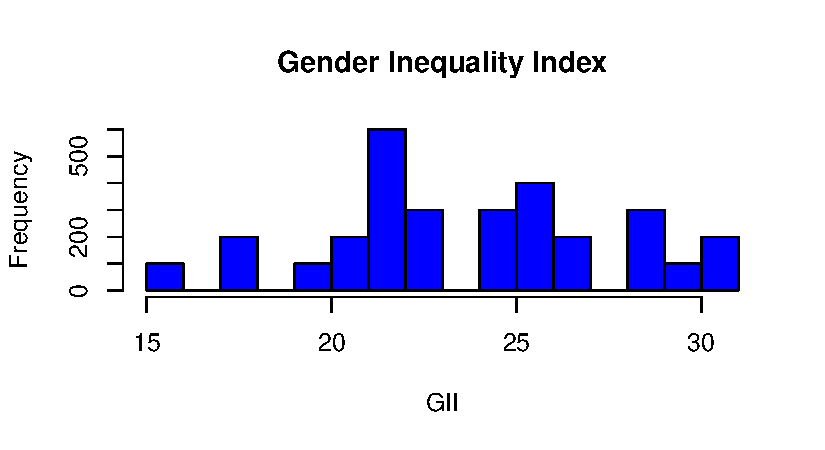
\includegraphics{quick-intro-R_files/figure-pdf/fig-hist-1.pdf}

}

\caption{\label{fig-hist}Histogram of Gender Inequality Index}

\end{figure}

\begin{tcolorbox}[enhanced jigsaw, bottomrule=.15mm, left=2mm, colframe=quarto-callout-tip-color-frame, title=\textcolor{quarto-callout-tip-color}{\faLightbulb}\hspace{0.5em}{Tip}, colback=white, leftrule=.75mm, coltitle=black, rightrule=.15mm, colbacktitle=quarto-callout-tip-color!10!white, opacityback=0, toptitle=1mm, toprule=.15mm, breakable, opacitybacktitle=0.6, bottomtitle=1mm, arc=.35mm, titlerule=0mm]

You often \emph{don't} need to use all of the options.
e.g.~\texttt{hist(mydata\$x)} will work just fine.

\end{tcolorbox}

\hypertarget{barplot}{%
\subsection{Barplot}\label{barplot}}

\begin{Shaded}
\begin{Highlighting}[]
\FunctionTok{barplot}\NormalTok{(}\FunctionTok{table}\NormalTok{(MICSsimulated}\SpecialCharTok{$}\NormalTok{aggression), }\CommentTok{\# what I\textquotesingle{}m graphing}
        \AttributeTok{main =} \StringTok{"Child Displays Aggression"}\NormalTok{, }\CommentTok{\# title}
        \AttributeTok{xlab =} \StringTok{"Aggression"}\NormalTok{, }\CommentTok{\# label for x axis}
        \AttributeTok{col =} \StringTok{"gold"}\NormalTok{) }\CommentTok{\# color}
\end{Highlighting}
\end{Shaded}

\begin{figure}[H]

{\centering 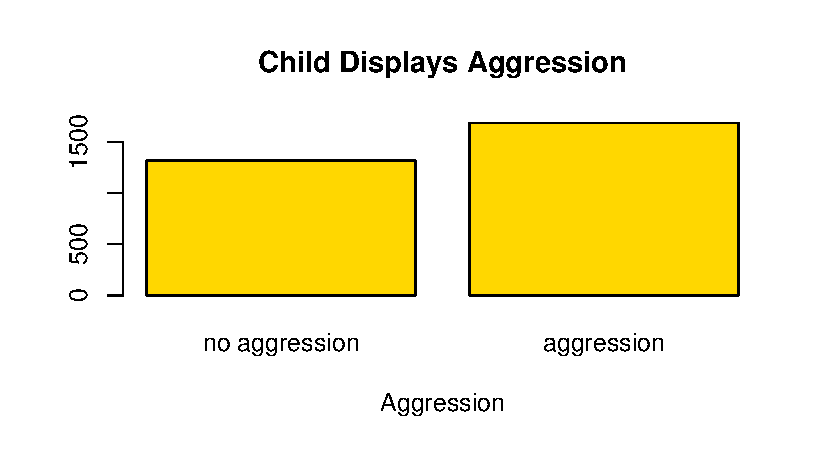
\includegraphics{quick-intro-R_files/figure-pdf/fig-barplot-1.pdf}

}

\caption{\label{fig-barplot}Barplot of Aggression}

\end{figure}

\begin{tcolorbox}[enhanced jigsaw, bottomrule=.15mm, left=2mm, colframe=quarto-callout-tip-color-frame, title=\textcolor{quarto-callout-tip-color}{\faLightbulb}\hspace{0.5em}{Tip}, colback=white, leftrule=.75mm, coltitle=black, rightrule=.15mm, colbacktitle=quarto-callout-tip-color!10!white, opacityback=0, toptitle=1mm, toprule=.15mm, breakable, opacitybacktitle=0.6, bottomtitle=1mm, arc=.35mm, titlerule=0mm]

You often \emph{don't} need to use all of the options.
e.g.~\texttt{barplot(table(mydata\$z))} will work just fine.

\end{tcolorbox}

\hypertarget{analyze-data-descriptive-statistics}{%
\section{Analyze Data: Descriptive
Statistics}\label{analyze-data-descriptive-statistics}}

\begin{Shaded}
\begin{Highlighting}[]
\FunctionTok{summary}\NormalTok{(mydata}\SpecialCharTok{$}\NormalTok{x) }\CommentTok{\# for continuous or factor variables}

\FunctionTok{table}\NormalTok{(mydata}\SpecialCharTok{$}\NormalTok{z) }\CommentTok{\# especially suitable for factor variables}
\end{Highlighting}
\end{Shaded}

\begin{Shaded}
\begin{Highlighting}[]
\FunctionTok{summary}\NormalTok{(MICSsimulated}\SpecialCharTok{$}\NormalTok{GII)}
\end{Highlighting}
\end{Shaded}

\begin{verbatim}
   Min. 1st Qu.  Median    Mean 3rd Qu.    Max. 
   15.0    22.0    24.0    24.2    27.0    31.0 
\end{verbatim}

\begin{Shaded}
\begin{Highlighting}[]
\FunctionTok{table}\NormalTok{(MICSsimulated}\SpecialCharTok{$}\NormalTok{aggression)}
\end{Highlighting}
\end{Shaded}

\begin{verbatim}

no aggression    aggression 
         1316          1684 
\end{verbatim}

\bookmarksetup{startatroot}

\hypertarget{a-quick-introduction-to-ggplot2}{%
\chapter{\texorpdfstring{A Quick Introduction To
\texttt{ggplot2}}{A Quick Introduction To ggplot2}}\label{a-quick-introduction-to-ggplot2}}

\hypertarget{why-use-ggplotmoreinformation}{%
\section[Why Use \texttt{ggplot}?]{\texorpdfstring{Why Use
\texttt{ggplot}?\footnote{More information can be found here:
  https://agrogan1.github.io/R/introduction-to-ggplot2/introduction-to-ggplot2.html}}{Why Use ggplot?}}\label{why-use-ggplotmoreinformation}}

A great deal of data analysis and visualization involves the same core
set of steps: get some data, clean it up a little, run some descriptive
statistics, run some bivariate statistics, create a graph or a
visualization. \textbf{ggplot2} can be an important part of a
replicable, automated, documented workflow for complex projects.

\[\text{have a question} \rightarrow \text{get data} \rightarrow \text{process and clean data} \rightarrow\]
\[\text{visualize data} \rightarrow \text{analyze data} \rightarrow \text{make conclusions}\]

Given the fact that we often want to apply the same core set of tasks to
new questions and new data, there are ways to overcome the steep
learning curve and learn a replicable set of commands that can be
applied to problem after problem.

\begin{quote}
The same 5 to 10 lines of ggplot2 code can often be tweaked over and
over again for multiple projects.
\end{quote}

\hypertarget{the-essential-idea-of-ggplot-is-simple}{%
\section{\texorpdfstring{The Essential Idea Of \texttt{ggplot} Is
Simple}{The Essential Idea Of ggplot Is Simple}}\label{the-essential-idea-of-ggplot-is-simple}}

There are 3 essential elements to any \texttt{ggplot} call:

\begin{enumerate}
\def\labelenumi{\arabic{enumi}.}
\tightlist
\item
  A reference to the data you are using.
\item
  An \emph{aesthetic} that tells \texttt{ggplot} which variables are
  being mapped to the \emph{x axis}, \emph{y axis}, (and often other
  attributes of the graph, such as the \emph{color}, * color fill\emph{,
  or even the }shape\emph{, }size\emph{, }transparency\emph{, or }line
  type*). Intuitively, the aesthetic can be thought of as \textbf{what
  you are graphing}.
\item
  A \emph{geom} or \emph{geometry} that tells ggplot about the basic
  structure of the graph. Intuitively, the geom can be thought of as
  \textbf{how you are graphing it}.
\end{enumerate}

You can also add other options, such as a \emph{graph title}, \emph{axis
labels} and \emph{overall theme} for the graph.

\hypertarget{get-started}{%
\section{Get Started}\label{get-started}}

\hypertarget{call-libraries}{%
\subsection{Call Libraries}\label{call-libraries}}

\begin{Shaded}
\begin{Highlighting}[]
\FunctionTok{library}\NormalTok{(ggplot2) }\CommentTok{\# beautiful graphs}

\FunctionTok{library}\NormalTok{(ggthemes) }\CommentTok{\# nice themes for ggplot2}
\end{Highlighting}
\end{Shaded}

\hypertarget{get-data-1}{%
\subsection{Get Data}\label{get-data-1}}

\begin{Shaded}
\begin{Highlighting}[]
\FunctionTok{load}\NormalTok{(}\StringTok{"./simulate{-}data/MICSsimulated.RData"}\NormalTok{) }\CommentTok{\# data in R format}
\end{Highlighting}
\end{Shaded}

\hypertarget{some-examplesvartype}{%
\section[Some Examples]{\texorpdfstring{Some
Examples\footnote{Changing variables from factor to numeric
  (e.g.~\texttt{aes(x\ =\ as.numeric(outcome))}), and \emph{vice versa}
  can sometimes be a simple solution that solves a lot of problems when
  you are trying to graph your variables.}}{Some Examples}}\label{some-examplesvartype}}

\hypertarget{one-continuous-variable}{%
\subsection{One Continuous Variable}\label{one-continuous-variable}}

\begin{Shaded}
\begin{Highlighting}[]
\CommentTok{\# anything that starts with a \textquotesingle{}\#\textquotesingle{} is a comment}

\FunctionTok{ggplot}\NormalTok{(MICSsimulated, }\CommentTok{\# the data I am using}
       \FunctionTok{aes}\NormalTok{(}\AttributeTok{x =}\NormalTok{ GII)) }\SpecialCharTok{+} \CommentTok{\# the variable I am using}
  \FunctionTok{geom\_histogram}\NormalTok{() }\CommentTok{\# how I am graphing it}
\end{Highlighting}
\end{Shaded}

\begin{figure}[H]

{\centering 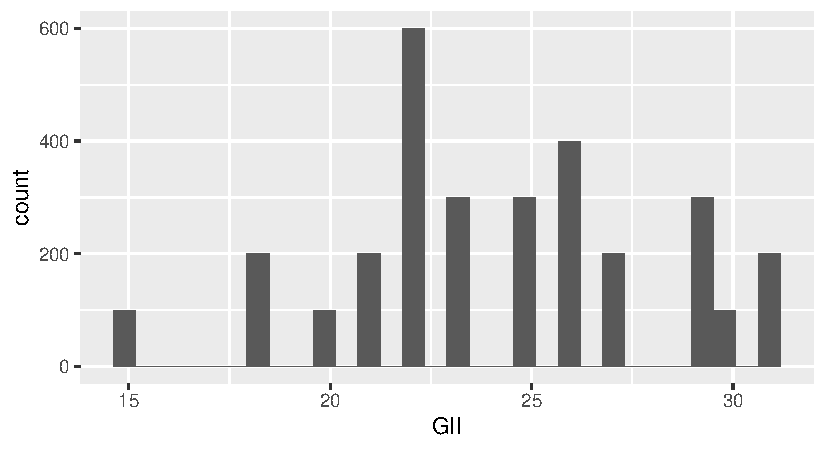
\includegraphics{quick-intro-ggplot2_files/figure-pdf/fig-ggplot-histogram-1.pdf}

}

\caption{\label{fig-ggplot-histogram}Histogram of Gender Inequality
Index}

\end{figure}

We can add color and a theme.

\begin{Shaded}
\begin{Highlighting}[]
\CommentTok{\# anything that starts with a \textquotesingle{}\#\textquotesingle{} is a comment}

\FunctionTok{ggplot}\NormalTok{(MICSsimulated, }\CommentTok{\# the data I am using}
       \FunctionTok{aes}\NormalTok{(}\AttributeTok{x =}\NormalTok{ GII)) }\SpecialCharTok{+} \CommentTok{\# the variable I am using}
  \FunctionTok{geom\_histogram}\NormalTok{(}\AttributeTok{fill =} \StringTok{"\#1CABE2"}\NormalTok{) }\SpecialCharTok{+} \CommentTok{\# how I am graphing it}
  \FunctionTok{theme\_minimal}\NormalTok{()}
\end{Highlighting}
\end{Shaded}

\begin{figure}[H]

{\centering 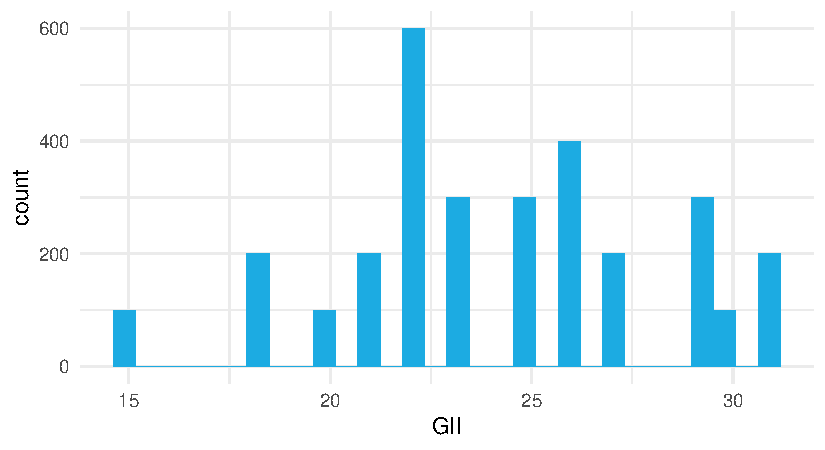
\includegraphics{quick-intro-ggplot2_files/figure-pdf/fig-ggplot-histogram-color-1.pdf}

}

\caption{\label{fig-ggplot-histogram-color}Histogram of Gender
Inequality Index}

\end{figure}

\hypertarget{one-categorical-variable}{%
\subsection{One Categorical Variable}\label{one-categorical-variable}}

Make sure R knows \texttt{aggression} is a categorical variable.

\begin{Shaded}
\begin{Highlighting}[]
\NormalTok{MICSsimulated}\SpecialCharTok{$}\NormalTok{aggression }\OtherTok{\textless{}{-}} 
  \FunctionTok{factor}\NormalTok{(MICSsimulated}\SpecialCharTok{$}\NormalTok{aggression, }\CommentTok{\# original numeric variable}
         \AttributeTok{levels =} \FunctionTok{c}\NormalTok{(}\DecValTok{0}\NormalTok{, }\DecValTok{1}\NormalTok{), }
         \AttributeTok{labels =} \FunctionTok{c}\NormalTok{(}\StringTok{"no aggression"}\NormalTok{, }\StringTok{"aggression"}\NormalTok{), }
         \AttributeTok{ordered =} \ConstantTok{TRUE}\NormalTok{) }\CommentTok{\# whether order matters}
\end{Highlighting}
\end{Shaded}

Now make the graph.

\begin{Shaded}
\begin{Highlighting}[]
\FunctionTok{ggplot}\NormalTok{(MICSsimulated, }\CommentTok{\# the data I am using}
       \FunctionTok{aes}\NormalTok{(}\AttributeTok{x =}\NormalTok{ aggression)) }\SpecialCharTok{+} \CommentTok{\# the variable I am using}
  \FunctionTok{geom\_bar}\NormalTok{() }\CommentTok{\# how I am graphing it}
\end{Highlighting}
\end{Shaded}

\begin{figure}[H]

{\centering 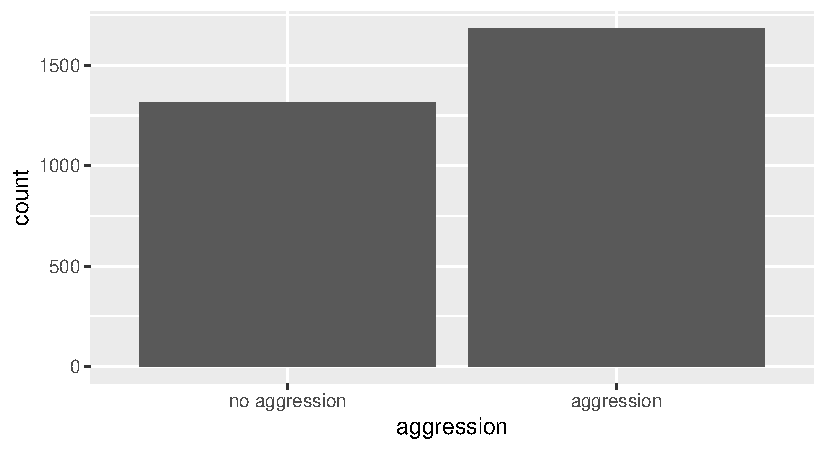
\includegraphics{quick-intro-ggplot2_files/figure-pdf/fig-ggplot-bar-1.pdf}

}

\caption{\label{fig-ggplot-bar}Bar Graph of Aggression}

\end{figure}

We can add color and a theme.\footnote{Notice how use of \texttt{fill}
  governs both the color fill in the graph below, as well as the legend
  that is produced in the graph.}

\begin{Shaded}
\begin{Highlighting}[]
\FunctionTok{ggplot}\NormalTok{(MICSsimulated, }\CommentTok{\# the data I am using}
       \FunctionTok{aes}\NormalTok{(}\AttributeTok{x =}\NormalTok{ aggression, }\CommentTok{\# x is aggression}
           \AttributeTok{fill =}\NormalTok{ aggression)) }\SpecialCharTok{+} \CommentTok{\# fill is also aggression}
  \FunctionTok{geom\_bar}\NormalTok{() }\SpecialCharTok{+} \CommentTok{\# how I am graphing it}
  \FunctionTok{theme\_minimal}\NormalTok{()}
\end{Highlighting}
\end{Shaded}

\begin{figure}[H]

{\centering 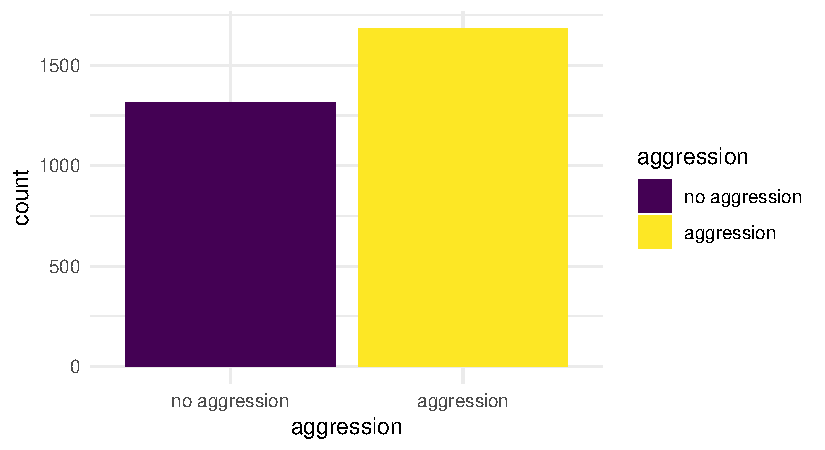
\includegraphics{quick-intro-ggplot2_files/figure-pdf/fig-ggplot-bar-color-1.pdf}

}

\caption{\label{fig-ggplot-bar-color}Bar Graph of Aggression}

\end{figure}

\hypertarget{make-a-more-complex-graphlegend2}{%
\section[Make a More Complex Graph]{\texorpdfstring{Make a More Complex
Graph\footnote{Notice how use of \texttt{fill} governs both the color
  fill in the graph below, as well as the legend that is produced in the
  graph.}}{Make a More Complex Graph}}\label{make-a-more-complex-graphlegend2}}

Make sure R knows \texttt{cd1} is a categorical variable.

\begin{Shaded}
\begin{Highlighting}[]
\NormalTok{MICSsimulated}\SpecialCharTok{$}\NormalTok{cd1 }\OtherTok{\textless{}{-}} 
  \FunctionTok{factor}\NormalTok{(MICSsimulated}\SpecialCharTok{$}\NormalTok{cd1, }\CommentTok{\# original numeric variable}
         \AttributeTok{levels =} \FunctionTok{c}\NormalTok{(}\DecValTok{0}\NormalTok{, }\DecValTok{1}\NormalTok{), }
         \AttributeTok{labels =} \FunctionTok{c}\NormalTok{(}\StringTok{"no spank"}\NormalTok{, }\StringTok{"spank"}\NormalTok{), }
         \AttributeTok{ordered =} \ConstantTok{TRUE}\NormalTok{) }\CommentTok{\# whether order matters}
\end{Highlighting}
\end{Shaded}

Now make the graph.

\begin{Shaded}
\begin{Highlighting}[]
\FunctionTok{ggplot}\NormalTok{(MICSsimulated, }\CommentTok{\# the data I am using}
       \FunctionTok{aes}\NormalTok{(}\AttributeTok{x =}\NormalTok{ cd1, }\CommentTok{\# x is spanking}
           \AttributeTok{fill =}\NormalTok{ aggression)) }\SpecialCharTok{+} \CommentTok{\# fill is aggression}
  \FunctionTok{geom\_bar}\NormalTok{(}\AttributeTok{position =} \FunctionTok{position\_dodge}\NormalTok{()) }\SpecialCharTok{+} \CommentTok{\# graph with "dodged" bars}
  \FunctionTok{labs}\NormalTok{(}\AttributeTok{title =} \StringTok{"Spanking and Aggression"}\NormalTok{, }
       \AttributeTok{x =} \StringTok{"spanking"}\NormalTok{, }
       \AttributeTok{y =} \StringTok{"count"}\NormalTok{) }\SpecialCharTok{+}
  \FunctionTok{scale\_fill\_manual}\NormalTok{(}\AttributeTok{values =} \FunctionTok{c}\NormalTok{(}\StringTok{"\#1CABE2"}\NormalTok{, }\CommentTok{\# UNICEF colors}
                               \StringTok{"\#D8D1C9"}\NormalTok{)) }\SpecialCharTok{+}
  \FunctionTok{theme\_minimal}\NormalTok{()  }\CommentTok{\# theme}
\end{Highlighting}
\end{Shaded}

\begin{figure}[H]

{\centering 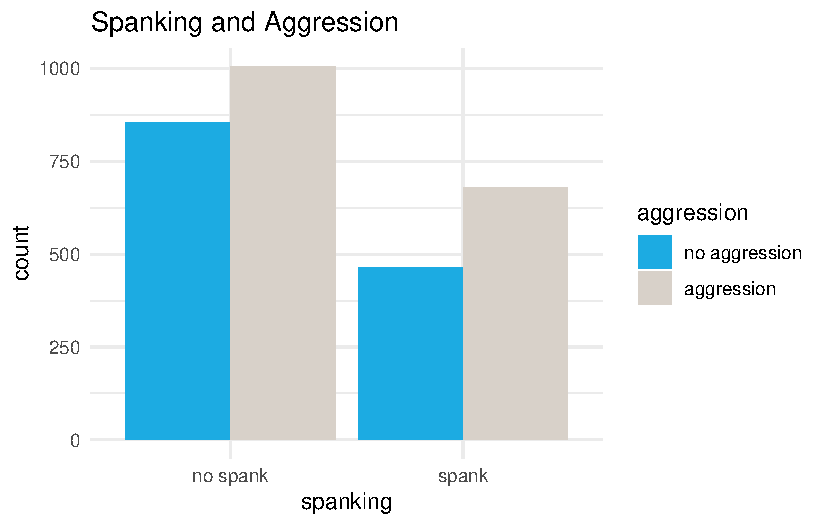
\includegraphics{quick-intro-ggplot2_files/figure-pdf/unnamed-chunk-8-1.pdf}

}

\end{figure}

An interactive tutorial to create this plot can be found
\href{https://agrogan1.github.io/globalfamilies-flipbook/}{here}.

\bookmarksetup{startatroot}

\hypertarget{quantitative-data-analysis}{%
\chapter{Quantitative Data Analysis}\label{quantitative-data-analysis}}

\hypertarget{introduction}{%
\section{Introduction}\label{introduction}}

A great deal of data analysis and visualization involves the same core
set of steps.

\[\text{have a question} \rightarrow \text{get data} \rightarrow \text{process and clean data} \rightarrow \text{analyze data}\]

\hypertarget{some-tools-for-analysis}{%
\section{Some Tools for Analysis}\label{some-tools-for-analysis}}

Below we describe some simple data cleaning with R. We begin, however,
by comparing several different tools for analysis including: Excel,
Google Sheets, R, and Stata.

\begin{longtable}[]{@{}
  >{\raggedright\arraybackslash}p{(\columnwidth - 10\tabcolsep) * \real{0.1139}}
  >{\raggedright\arraybackslash}p{(\columnwidth - 10\tabcolsep) * \real{0.1646}}
  >{\raggedright\arraybackslash}p{(\columnwidth - 10\tabcolsep) * \real{0.1646}}
  >{\raggedright\arraybackslash}p{(\columnwidth - 10\tabcolsep) * \real{0.1899}}
  >{\raggedright\arraybackslash}p{(\columnwidth - 10\tabcolsep) * \real{0.1772}}
  >{\raggedright\arraybackslash}p{(\columnwidth - 10\tabcolsep) * \real{0.1899}}@{}}
\toprule\noalign{}
\begin{minipage}[b]{\linewidth}\raggedright
Tool
\end{minipage} & \begin{minipage}[b]{\linewidth}\raggedright
Cost
\end{minipage} & \begin{minipage}[b]{\linewidth}\raggedright
Ease of Use
\end{minipage} & \begin{minipage}[b]{\linewidth}\raggedright
Analysis Capabilities
\end{minipage} & \begin{minipage}[b]{\linewidth}\raggedright
Suitability for Large Data
\end{minipage} & \begin{minipage}[b]{\linewidth}\raggedright
Keep Track of Complicated Workflows
\end{minipage} \\
\midrule\noalign{}
\endhead
\bottomrule\noalign{}
\endlastfoot
Excel & Comes installed on many computers & Easy & Limited & Difficult
when N \textgreater{} 100 & Difficult to Impossible \\
Google Sheets & Free with a Google account & Easy & Limited & Difficult
when N \textgreater{} 100 & Difficult to Impossible \\
R & Free & Challenging & Extensive & Excellent with large datasets &
Yes, with script \\
Stata & Some cost & Learning Curve but Intuitive & Extensive & Excellent
with large datasets & Yes, with command file \\
\end{longtable}

\hypertarget{working-with-r}{%
\section{Working With R}\label{working-with-r}}

\hypertarget{our-data}{%
\subsection{Our Data}\label{our-data}}

We take a look at our \emph{simulated} data.

\begin{Shaded}
\begin{Highlighting}[]
\FunctionTok{load}\NormalTok{(}\StringTok{"./simulate{-}data/MICSsimulated.RData"}\NormalTok{) }\CommentTok{\# data in R format}

\NormalTok{labelled}\SpecialCharTok{::}\FunctionTok{look\_for}\NormalTok{(MICSsimulated) }\CommentTok{\# look at data}
\end{Highlighting}
\end{Shaded}

\begin{verbatim}
 pos variable   label                   col_type missing values
 1   id         id                      int      0             
 2   country    country                 int      0             
 3   GII        Gender Inequality Index int      0             
 4   HDI        Human Development Index int      0             
 5   cd1        spank                   int      0             
 6   cd2        beat                    int      0             
 7   cd3        shout                   int      0             
 8   cd4        explain                 int      0             
 9   aggression aggression              int      0             
\end{verbatim}

\hypertarget{cleaning-data}{%
\subsection{Cleaning Data}\label{cleaning-data}}

There are some basic data cleaning steps that are common to many
projects.

\begin{itemize}
\tightlist
\item
  Only keep the variables of interest. Section~\ref{sec-onlykeep}
\item
  Add variable labels (if we can). Section~\ref{sec-addvarlabels}
\item
  Add value labels (if we can). Section~\ref{sec-addvaluelabels}
\item
  Recode outliers, values that are errors, or values that should be
  coded as missing Section~\ref{sec-recodes}
\end{itemize}

\begin{quote}
Much of R's functionality is accomplished through writing \emph{code},
that is saved in a \emph{script}. Notice how--as our tasks get more and
more complicated--the saved script provides documentation for the
decisions that we have made with the data.
\end{quote}

\hypertarget{sec-onlykeep}{%
\subsubsection{Only keep the variables of
interest.}\label{sec-onlykeep}}

\begin{quote}
We can easily accomplish this with the \texttt{subset} function
\end{quote}

\begin{Shaded}
\begin{Highlighting}[]
\NormalTok{mynewdata }\OtherTok{\textless{}{-}} \FunctionTok{subset}\NormalTok{(MICSsimulated,}
                    \AttributeTok{select =} \FunctionTok{c}\NormalTok{(id, country, aggression))}
\end{Highlighting}
\end{Shaded}

\begin{Shaded}
\begin{Highlighting}[]
\FunctionTok{head}\NormalTok{(mynewdata)}
\end{Highlighting}
\end{Shaded}

\begin{verbatim}
  id country aggression
1  1       1          1
2  2       1          1
3  3       1          1
4  4       1          1
5  5       1          0
6  6       1          1
\end{verbatim}

\hypertarget{sec-addvarlabels}{%
\subsubsection{Add variable labels (if we
can).}\label{sec-addvarlabels}}

\begin{quote}
Adding \emph{variable labels} is still somewhat new in R. The
\texttt{labelled} library allows us to add or change variable labels.
However, not every library in R recognizes \emph{variable labels}.
\end{quote}

\begin{Shaded}
\begin{Highlighting}[]
\FunctionTok{library}\NormalTok{(labelled)}

\FunctionTok{var\_label}\NormalTok{(MICSsimulated}\SpecialCharTok{$}\NormalTok{id) }\OtherTok{\textless{}{-}} \StringTok{"id"}

\FunctionTok{var\_label}\NormalTok{(MICSsimulated}\SpecialCharTok{$}\NormalTok{country) }\OtherTok{\textless{}{-}} \StringTok{"country"}

\FunctionTok{var\_label}\NormalTok{(MICSsimulated}\SpecialCharTok{$}\NormalTok{cd4) }\OtherTok{\textless{}{-}} \StringTok{"explain"}
\end{Highlighting}
\end{Shaded}

\hypertarget{sec-addvaluelabels}{%
\subsubsection{Add value labels (if we can).}\label{sec-addvaluelabels}}

\begin{quote}
In contrast, \emph{value labels} are straightforward in R, and can be
accomplished by creating a \emph{factor variable}. Below we demonstrate
how to do this with the happy variable.
\end{quote}

\begin{Shaded}
\begin{Highlighting}[]
\NormalTok{MICSsimulated}\SpecialCharTok{$}\NormalTok{cd4 }\OtherTok{\textless{}{-}} \FunctionTok{factor}\NormalTok{(MICSsimulated}\SpecialCharTok{$}\NormalTok{cd4,}
                             \AttributeTok{levels =} \FunctionTok{c}\NormalTok{(}\DecValTok{0}\NormalTok{, }\DecValTok{1}\NormalTok{),}
                             \AttributeTok{labels =} \FunctionTok{c}\NormalTok{(}\StringTok{"Did not explain"}\NormalTok{,}
                                        \StringTok{"Explained"}\NormalTok{))}
\end{Highlighting}
\end{Shaded}

\begin{Shaded}
\begin{Highlighting}[]
\FunctionTok{head}\NormalTok{(MICSsimulated)}
\end{Highlighting}
\end{Shaded}

\begin{verbatim}
  id country GII HDI cd1 cd2 cd3             cd4 aggression
1  1       1  20  24   0   0   1       Explained          1
2  2       1  20  24   0   0   1       Explained          1
3  3       1  20  24   0   0   1       Explained          1
4  4       1  20  24   0   0   0 Did not explain          1
5  5       1  20  24   1   0   1       Explained          0
6  6       1  20  24   0   0   1       Explained          1
\end{verbatim}

\hypertarget{sec-recodes}{%
\subsubsection{Recode outliers, values that are errors, or values that
should be coded as missing.}\label{sec-recodes}}

\begin{quote}
We can easily accomplish this using Base R's syntax for recoding:
\texttt{data\$variable{[}rule{]}\ \textless{}-\ newvalue}.
\end{quote}

\begin{Shaded}
\begin{Highlighting}[]
\NormalTok{MICSsimulated}\SpecialCharTok{$}\NormalTok{aggression[MICSsimulated}\SpecialCharTok{$}\NormalTok{aggression }\SpecialCharTok{\textgreater{}} \DecValTok{1}\NormalTok{] }\OtherTok{\textless{}{-}} \ConstantTok{NA} \CommentTok{\# recode \textgreater{} 1 to NA}

\NormalTok{MICSsimulated}\SpecialCharTok{$}\NormalTok{GII[MICSsimulated}\SpecialCharTok{$}\NormalTok{GII }\SpecialCharTok{\textgreater{}} \DecValTok{100}\NormalTok{] }\OtherTok{\textless{}{-}} \ConstantTok{NA} \CommentTok{\# recode \textgreater{} 100 to NA}
\end{Highlighting}
\end{Shaded}

\begin{Shaded}
\begin{Highlighting}[]
\FunctionTok{head}\NormalTok{(MICSsimulated)}
\end{Highlighting}
\end{Shaded}

\begin{verbatim}
  id country GII HDI cd1 cd2 cd3             cd4 aggression
1  1       1  20  24   0   0   1       Explained          1
2  2       1  20  24   0   0   1       Explained          1
3  3       1  20  24   0   0   1       Explained          1
4  4       1  20  24   0   0   0 Did not explain          1
5  5       1  20  24   1   0   1       Explained          0
6  6       1  20  24   0   0   1       Explained          1
\end{verbatim}

\hypertarget{simple-analysis}{%
\subsection{Simple Analysis}\label{simple-analysis}}

Our first step in analysis is to discover what kind of variables we
have. We need to make a distinction between \emph{continuous variables}
that measure things like mental health or neighborhood safety, or age,
and \emph{categorical variables} that measure non-ordered categories
like religious identity or gender identity.

\begin{itemize}
\tightlist
\item
  For continuous variables, it is most appropriate to take the
  \emph{average} or \emph{mean}.
\item
  For categorical variables, it is most appropriate to generate a
  \emph{frequency table}.
\end{itemize}

\begin{quote}
As a mostly command based language, R relies on the idea of
\texttt{do\_something(dataset\$variable)}.
\end{quote}

\begin{Shaded}
\begin{Highlighting}[]
\FunctionTok{summary}\NormalTok{(MICSsimulated}\SpecialCharTok{$}\NormalTok{GII) }\CommentTok{\# descriptive statistics for GII}
\end{Highlighting}
\end{Shaded}

\begin{verbatim}
   Min. 1st Qu.  Median    Mean 3rd Qu.    Max. 
   15.0    22.0    24.0    24.2    27.0    31.0 
\end{verbatim}

\begin{Shaded}
\begin{Highlighting}[]
\FunctionTok{table}\NormalTok{(MICSsimulated}\SpecialCharTok{$}\NormalTok{cd4) }\CommentTok{\# frequency table of cd4}
\end{Highlighting}
\end{Shaded}

\begin{verbatim}

Did not explain       Explained 
            674            2326 
\end{verbatim}

\bookmarksetup{startatroot}

\hypertarget{references}{%
\chapter*{References}\label{references}}
\addcontentsline{toc}{chapter}{References}

\markboth{References}{References}

\hypertarget{refs}{}
\begin{CSLReferences}{1}{0}
\leavevmode\vadjust pre{\hypertarget{ref-Kreft1998}{}}%
Kreft, I., \& de Leeuw, J. (1998). \emph{Introducing multilevel
modeling}. SAGE Publications.
\url{https://doi.org/10.4135/9781849209366}

\leavevmode\vadjust pre{\hypertarget{ref-Luke2004}{}}%
Luke, D. (2004). \emph{Multilevel modeling}. SAGE Publications, Inc.
\url{https://doi.org/10.4135/9781412985147}

\leavevmode\vadjust pre{\hypertarget{ref-RabeHesketh2022}{}}%
Rabe-Hesketh, S., \& Skrondal, A. (2022). Multilevel and longitudinal
modeling using {S}tata. In \emph{Stata Press} (4th ed.). Stata Press.

\leavevmode\vadjust pre{\hypertarget{ref-Raudenbush2002}{}}%
Raudenbush, S. W., \& Bryk, A. S. (2002). \emph{Hierarchical linear
models: Applications and data analysis methods} (pp. xxiv, 485 p.). Sage
Publications.

\leavevmode\vadjust pre{\hypertarget{ref-Singer2003}{}}%
Singer, J. D., \& Willett, J. B. (2003). Applied longitudinal data
analysis : Modeling change and event occurrence. In \emph{Applied
longitudinal data analysis : modeling change and event occurrence}.
Oxford University Press.

\leavevmode\vadjust pre{\hypertarget{ref-UNDPHDI}{}}%
United Nations Development Program. (2022). \emph{{Human Development
Index (HDI)}}.
\url{https://hdr.undp.org/data-center/human-development-index\#/indicies/HDI}

\leavevmode\vadjust pre{\hypertarget{ref-UNDPGII}{}}%
United Nations Development Program. (2023). \emph{{Gender Inequality
Index (GII)}}.
\url{https://hdr.undp.org/data-center/thematic-composite-indices/gender-inequality-index\#/indicies/GII}

\end{CSLReferences}

\cleardoublepage
\phantomsection
\addcontentsline{toc}{part}{Appendices}
\appendix

\hypertarget{simulating-mics-data}{%
\chapter{Simulating MICS Data}\label{simulating-mics-data}}

This appendix details the process of creating the simulated MICS data
that is employed in the examples on this website.

MICS data are freely available, but usage of MICS requires completing a
user agreement, and registering for a user account, on the MICS website,
and thus MICS data should not be shared openly on a public website.

This Appendix is highly technical. It is not necessary to understand
this Appendix to benefit from the rest of this website. However, the
details of creating this simulated data may be of interest to some
users.

\hypertarget{call-relevant-libraries}{%
\section{Call Relevant Libraries}\label{call-relevant-libraries}}

We need to call a number of relevant R libraries to simulate the data.

\begin{Shaded}
\begin{Highlighting}[]
\FunctionTok{library}\NormalTok{(tibble) }\CommentTok{\# new dataframes}

\FunctionTok{library}\NormalTok{(ggplot2) }\CommentTok{\# nifty graphs}

\FunctionTok{library}\NormalTok{(labelled) }\CommentTok{\# labels}

\FunctionTok{library}\NormalTok{(haven) }\CommentTok{\# write Stata}

\FunctionTok{library}\NormalTok{(tidyr) }\CommentTok{\# tidy data}

\FunctionTok{library}\NormalTok{(dplyr) }\CommentTok{\# wrangle data}

\FunctionTok{library}\NormalTok{(lme4) }\CommentTok{\# multilevel models}

\FunctionTok{library}\NormalTok{(sjPlot) }\CommentTok{\# nice tables for MLM}

\FunctionTok{library}\NormalTok{(pander) }\CommentTok{\# nice tables}
\end{Highlighting}
\end{Shaded}

\hypertarget{setup-some-basic-parameters-of-the-data}{%
\section{Setup Some Basic Parameters of the
Data}\label{setup-some-basic-parameters-of-the-data}}

Because simulation is a random process, we set a \emph{random seed} so
that the simulation produces the same data set each time it is run.

We are going to simulate data with 30 countries, and 100 individuals per
country.

\begin{Shaded}
\begin{Highlighting}[]
\FunctionTok{set.seed}\NormalTok{(}\DecValTok{1234}\NormalTok{) }\CommentTok{\# random seed}

\NormalTok{N\_countries }\OtherTok{\textless{}{-}} \DecValTok{30} \CommentTok{\# number of countries}

\NormalTok{N }\OtherTok{\textless{}{-}} \DecValTok{100} \CommentTok{\# sample size / country}
\end{Highlighting}
\end{Shaded}

\hypertarget{simulate-data-based-on-mics}{%
\section{Simulate Data Based on
MICS}\label{simulate-data-based-on-mics}}

This is multilevel data where individuals are nested, or clustered,
inside countries. Excellent technical and pedagogical discussions of
multilevel models can be found in Raudenbush \& Bryk (2002), Singer \&
Willett (2003), Rabe-Hesketh \& Skrondal (2022), Luke (2004), and Kreft
\& de Leeuw (1998).

\hypertarget{level-2}{%
\subsection{Level 2}\label{level-2}}

Simulating the second level of the data is relatively easy. We simply
need to provide the number of countries, and then generate random
effects for each country. Random effects are discussed in the above
references, but essentially represent country level differences in the
data.

We also create \texttt{GII}, a \emph{Gender Inequality Index} (United
Nations Development Program, 2023) variable, and \texttt{HDI}, a measure
of the \emph{Human Development Index} (United Nations Development
Program, 2022), since these are country level, or Level 2 variables.

\begin{Shaded}
\begin{Highlighting}[]
\NormalTok{country }\OtherTok{\textless{}{-}} \FunctionTok{seq}\NormalTok{(}\DecValTok{1}\SpecialCharTok{:}\NormalTok{N\_countries) }\CommentTok{\# sequence 1 to 30}

\NormalTok{GII }\OtherTok{\textless{}{-}} \FunctionTok{rbinom}\NormalTok{(N\_countries, }\DecValTok{100}\NormalTok{, .}\DecValTok{25}\NormalTok{) }\CommentTok{\# gender inequality index}

\NormalTok{HDI }\OtherTok{\textless{}{-}} \FunctionTok{rbinom}\NormalTok{(N\_countries, }\DecValTok{100}\NormalTok{, .}\DecValTok{25}\NormalTok{) }\CommentTok{\# Human Development Index}

\NormalTok{u0 }\OtherTok{\textless{}{-}} \FunctionTok{rnorm}\NormalTok{(N\_countries, }\DecValTok{0}\NormalTok{, .}\DecValTok{25}\NormalTok{) }\CommentTok{\# random intercept}

\NormalTok{u1 }\OtherTok{\textless{}{-}} \FunctionTok{rnorm}\NormalTok{(N\_countries, }\DecValTok{0}\NormalTok{, .}\DecValTok{05}\NormalTok{) }\CommentTok{\# random slope}

\NormalTok{randomeffects }\OtherTok{\textless{}{-}} \FunctionTok{data.frame}\NormalTok{(country, }
\NormalTok{                            GII, }
\NormalTok{                            HDI, }
\NormalTok{                            u0, }
\NormalTok{                            u1) }\CommentTok{\# dataframe of random effects}
\end{Highlighting}
\end{Shaded}

\hypertarget{level-1}{%
\subsection{Level 1}\label{level-1}}

Simulating the Level 1 data is more complex.

We \texttt{uncount} the data by 100 to create 100 observations for each
country. We then create an \texttt{id} number.

We create randomly simulated parental discipline variables with
proportions similar to those in MICS.

Lastly, we need to create the dependent variable. Because this is a
dichotomous outcome, the process is somewhat complex. We need to craete
a linear combination \texttt{z}, using regression weights derived from
MICS. We then calculate predicted probabilities, and lastly generate a
dichotomous \texttt{aggression} outcome from those probabilities.

\begin{Shaded}
\begin{Highlighting}[]
\NormalTok{MICSsimulated }\OtherTok{\textless{}{-}}\NormalTok{ randomeffects }\SpecialCharTok{\%\textgreater{}\%} 
  \FunctionTok{uncount}\NormalTok{(N) }\SpecialCharTok{\%\textgreater{}\%} \CommentTok{\# N individuals / country}
  \FunctionTok{mutate}\NormalTok{(}\AttributeTok{id =} \FunctionTok{row\_number}\NormalTok{()) }\SpecialCharTok{\%\textgreater{}\%} \CommentTok{\# unique id}
  \FunctionTok{mutate}\NormalTok{(}\AttributeTok{cd1 =} \FunctionTok{rbinom}\NormalTok{(N }\SpecialCharTok{*}\NormalTok{ N\_countries, }\DecValTok{1}\NormalTok{, .}\DecValTok{38}\NormalTok{), }\CommentTok{\# spank}
         \AttributeTok{cd2 =} \FunctionTok{rbinom}\NormalTok{(N }\SpecialCharTok{*}\NormalTok{ N\_countries, }\DecValTok{1}\NormalTok{, .}\DecValTok{05}\NormalTok{), }\CommentTok{\# beat}
         \AttributeTok{cd3 =} \FunctionTok{rbinom}\NormalTok{(N }\SpecialCharTok{*}\NormalTok{ N\_countries, }\DecValTok{1}\NormalTok{, .}\DecValTok{64}\NormalTok{), }\CommentTok{\# shout}
         \AttributeTok{cd4 =} \FunctionTok{rbinom}\NormalTok{(N }\SpecialCharTok{*}\NormalTok{ N\_countries, }\DecValTok{1}\NormalTok{, .}\DecValTok{78}\NormalTok{)) }\SpecialCharTok{\%\textgreater{}\%} \CommentTok{\# explain}
  \FunctionTok{mutate}\NormalTok{(}\AttributeTok{z =} \DecValTok{0} \SpecialCharTok{+} \CommentTok{\# linear combination based on MICS}
\NormalTok{           .}\DecValTok{01} \SpecialCharTok{*}\NormalTok{ GII }\SpecialCharTok{+}
\NormalTok{           .}\DecValTok{23} \SpecialCharTok{*}\NormalTok{ cd1 }\SpecialCharTok{+}
\NormalTok{           .}\DecValTok{52} \SpecialCharTok{*}\NormalTok{ cd2 }\SpecialCharTok{+}
\NormalTok{           .}\DecValTok{42} \SpecialCharTok{*}\NormalTok{ cd3 }\SpecialCharTok{+}
           \SpecialCharTok{{-}}\NormalTok{.}\DecValTok{21} \SpecialCharTok{*}\NormalTok{ cd4 }\SpecialCharTok{+} 
\NormalTok{           u0) }\SpecialCharTok{\%\textgreater{}\%}
  \FunctionTok{mutate}\NormalTok{(}\AttributeTok{p =} \FunctionTok{exp}\NormalTok{(z) }\SpecialCharTok{/}\NormalTok{ (}\DecValTok{1} \SpecialCharTok{+} \FunctionTok{exp}\NormalTok{(z))) }\SpecialCharTok{\%\textgreater{}\%} \CommentTok{\# probability}
  \FunctionTok{mutate}\NormalTok{(}\AttributeTok{aggression =} \FunctionTok{rbinom}\NormalTok{(N }\SpecialCharTok{*}\NormalTok{ N\_countries, }\DecValTok{1}\NormalTok{, p)) }\SpecialCharTok{\%\textgreater{}\%} \CommentTok{\# binomial y}
  \FunctionTok{select}\NormalTok{(id, country, GII, HDI,}
\NormalTok{         cd1, cd2, cd3, cd4, }
\NormalTok{         aggression)}
\end{Highlighting}
\end{Shaded}

\hypertarget{variable-labels}{%
\subsection{Variable Labels}\label{variable-labels}}

We add variable labels to the data which will help us to understand the
data as we analyze it.

\begin{Shaded}
\begin{Highlighting}[]
\FunctionTok{var\_label}\NormalTok{(MICSsimulated}\SpecialCharTok{$}\NormalTok{id) }\OtherTok{\textless{}{-}} \StringTok{"id"}

\FunctionTok{var\_label}\NormalTok{(MICSsimulated}\SpecialCharTok{$}\NormalTok{country) }\OtherTok{\textless{}{-}} \StringTok{"country"}

\FunctionTok{var\_label}\NormalTok{(MICSsimulated}\SpecialCharTok{$}\NormalTok{GII) }\OtherTok{\textless{}{-}} \StringTok{"Gender Inequality Index"}

\FunctionTok{var\_label}\NormalTok{(MICSsimulated}\SpecialCharTok{$}\NormalTok{HDI) }\OtherTok{\textless{}{-}} \StringTok{"Human Development Index"}

\FunctionTok{var\_label}\NormalTok{(MICSsimulated}\SpecialCharTok{$}\NormalTok{cd1) }\OtherTok{\textless{}{-}} \StringTok{"spank"}

\FunctionTok{var\_label}\NormalTok{(MICSsimulated}\SpecialCharTok{$}\NormalTok{cd2) }\OtherTok{\textless{}{-}} \StringTok{"beat"}

\FunctionTok{var\_label}\NormalTok{(MICSsimulated}\SpecialCharTok{$}\NormalTok{cd3) }\OtherTok{\textless{}{-}} \StringTok{"shout"}

\FunctionTok{var\_label}\NormalTok{(MICSsimulated}\SpecialCharTok{$}\NormalTok{cd4) }\OtherTok{\textless{}{-}} \StringTok{"explain"}

\FunctionTok{var\_label}\NormalTok{(MICSsimulated}\SpecialCharTok{$}\NormalTok{aggression) }\OtherTok{\textless{}{-}} \StringTok{"aggression"}
\end{Highlighting}
\end{Shaded}

\begin{Shaded}
\begin{Highlighting}[]
\FunctionTok{pander}\NormalTok{(labelled}\SpecialCharTok{::}\FunctionTok{look\_for}\NormalTok{(MICSsimulated)[}\DecValTok{1}\SpecialCharTok{:}\DecValTok{4}\NormalTok{]) }\CommentTok{\# list out variable labels}
\end{Highlighting}
\end{Shaded}

\hypertarget{tbl-varlabels}{}
\begin{longtable}[]{@{}
  >{\centering\arraybackslash}p{(\columnwidth - 6\tabcolsep) * \real{0.0833}}
  >{\centering\arraybackslash}p{(\columnwidth - 6\tabcolsep) * \real{0.1806}}
  >{\centering\arraybackslash}p{(\columnwidth - 6\tabcolsep) * \real{0.3611}}
  >{\centering\arraybackslash}p{(\columnwidth - 6\tabcolsep) * \real{0.1528}}@{}}
\caption{\label{tbl-varlabels}Variable Labels}\tabularnewline
\toprule\noalign{}
\begin{minipage}[b]{\linewidth}\centering
pos
\end{minipage} & \begin{minipage}[b]{\linewidth}\centering
variable
\end{minipage} & \begin{minipage}[b]{\linewidth}\centering
label
\end{minipage} & \begin{minipage}[b]{\linewidth}\centering
col\_type
\end{minipage} \\
\midrule\noalign{}
\endfirsthead
\toprule\noalign{}
\begin{minipage}[b]{\linewidth}\centering
pos
\end{minipage} & \begin{minipage}[b]{\linewidth}\centering
variable
\end{minipage} & \begin{minipage}[b]{\linewidth}\centering
label
\end{minipage} & \begin{minipage}[b]{\linewidth}\centering
col\_type
\end{minipage} \\
\midrule\noalign{}
\endhead
\bottomrule\noalign{}
\endlastfoot
1 & id & id & int \\
2 & country & country & int \\
3 & GII & Gender Inequality Index & int \\
4 & HDI & Human Development Index & int \\
5 & cd1 & spank & int \\
6 & cd2 & beat & int \\
7 & cd3 & shout & int \\
8 & cd4 & explain & int \\
9 & aggression & aggression & int \\
\end{longtable}

\hypertarget{explore-the-simulated-data-with-a-graph}{%
\section{Explore The Simulated Data With A
Graph}\label{explore-the-simulated-data-with-a-graph}}

Exploring the simulated data with a graph helps us to ensure that we
have simulated plausible data.

\begin{Shaded}
\begin{Highlighting}[]
\FunctionTok{ggplot}\NormalTok{(MICSsimulated,}
       \FunctionTok{aes}\NormalTok{(}\AttributeTok{x =}\NormalTok{ cd1, }\CommentTok{\# x is spanking}
           \AttributeTok{y =}\NormalTok{ aggression, }\CommentTok{\# y is aggression}
           \AttributeTok{color =} \FunctionTok{factor}\NormalTok{(country))) }\SpecialCharTok{+} \CommentTok{\# color is country}
  \FunctionTok{geom\_smooth}\NormalTok{(}\AttributeTok{method =} \StringTok{"glm"}\NormalTok{, }\CommentTok{\# glm smoother}
              \AttributeTok{method.args =} \FunctionTok{list}\NormalTok{(}\AttributeTok{family =} \StringTok{"binomial"}\NormalTok{),}
              \AttributeTok{alpha =}\NormalTok{ .}\DecValTok{1}\NormalTok{) }\SpecialCharTok{+} \CommentTok{\# transparency for CI\textquotesingle{}s}
  \FunctionTok{labs}\NormalTok{(}\AttributeTok{title =} \StringTok{"Aggression as a Function of Spanking"}\NormalTok{,}
       \AttributeTok{x =} \StringTok{"spank"}\NormalTok{,}
       \AttributeTok{y =} \StringTok{"aggression"}\NormalTok{) }\SpecialCharTok{+}
  \FunctionTok{scale\_color\_viridis\_d}\NormalTok{(}\AttributeTok{name =} \StringTok{"Country"}\NormalTok{) }\SpecialCharTok{+} \CommentTok{\# nice colors}
  \FunctionTok{theme\_minimal}\NormalTok{()}
\end{Highlighting}
\end{Shaded}

\begin{figure}[H]

{\centering 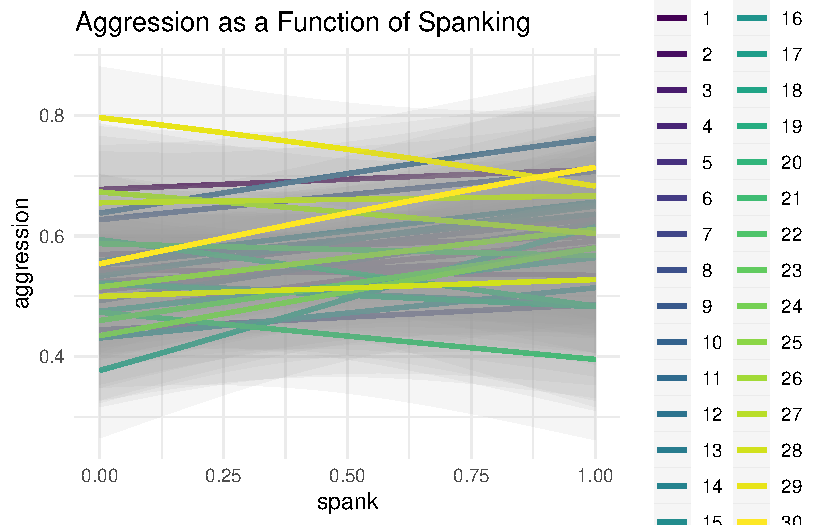
\includegraphics{simulate-data_files/figure-pdf/fig-p1-1.pdf}

}

\caption{\label{fig-p1}Graph of Simulated Data}

\end{figure}

\hypertarget{explore-the-simulated-data-with-a-logistic-regression}{%
\section{Explore The Simulated Data With A Logistic
Regression}\label{explore-the-simulated-data-with-a-logistic-regression}}

Similarly, exploring the data with a logistic regression confirms that
we have created plausible data.

\begin{Shaded}
\begin{Highlighting}[]
\NormalTok{fit1 }\OtherTok{\textless{}{-}} \FunctionTok{glmer}\NormalTok{(aggression }\SpecialCharTok{\textasciitilde{}}\NormalTok{ cd1 }\SpecialCharTok{+}\NormalTok{ cd2 }\SpecialCharTok{+}\NormalTok{ cd3 }\SpecialCharTok{+}\NormalTok{ cd4 }\SpecialCharTok{+}\NormalTok{ GII }\SpecialCharTok{+}
\NormalTok{                (}\DecValTok{1} \SpecialCharTok{|}\NormalTok{ country), }
              \AttributeTok{family =} \StringTok{"binomial"}\NormalTok{,}
              \AttributeTok{data =}\NormalTok{ MICSsimulated,}
              \AttributeTok{control =} \FunctionTok{glmerControl}\NormalTok{(}\AttributeTok{optimizer =}\StringTok{"bobyqa"}\NormalTok{))}

\FunctionTok{tab\_model}\NormalTok{(fit1, }\CommentTok{\# nice table}
          \AttributeTok{transform =} \ConstantTok{NULL}\NormalTok{) }\CommentTok{\# untransformed estimates}
\end{Highlighting}
\end{Shaded}

\begin{table}

\caption{\textbf{?(caption)}}

\end{table}

\hypertarget{write-data-to-various-formats}{%
\section{Write data to various
formats}\label{write-data-to-various-formats}}

Lastly, we write the data out to various formats: R, Stata, and SPSS.

\begin{Shaded}
\begin{Highlighting}[]
\FunctionTok{save}\NormalTok{(MICSsimulated, }
     \AttributeTok{file =} \StringTok{"./simulate{-}data/MICSsimulated.RData"}\NormalTok{) }\CommentTok{\# R}

\FunctionTok{write\_dta}\NormalTok{(MICSsimulated, }
          \StringTok{"./simulate{-}data/MICSsimulated.dta"}\NormalTok{) }\CommentTok{\# Stata}

\FunctionTok{write\_sav}\NormalTok{(MICSsimulated, }
          \StringTok{"./simulate{-}data/MICSsimulated.sav"}\NormalTok{) }\CommentTok{\# SPSS}
\end{Highlighting}
\end{Shaded}




\end{document}
